\documentclass[10pt,a4paper]{article}
\usepackage[utf8]{inputenc}
\usepackage[T1]{fontenc}
\usepackage[spanish,es-tabla]{babel}
\usepackage{lmodern}
\usepackage[left=2cm,right=2cm,top=2cm,bottom=2cm]{geometry}
\usepackage{graphicx}
\usepackage{booktabs}
\usepackage{array}
\usepackage{caption}
\usepackage{xcolor}
\usepackage{listings}
\usepackage{microtype}
\usepackage{hyperref}
\usepackage{fancyhdr}
\usepackage{enumitem}
\usepackage{float}

\hypersetup{colorlinks=true,linkcolor=black,urlcolor=blue!45!black,citecolor=black,pdftitle={Tarea 2: Protocolo MySQL y analisis de trafico}}
\setlength{\parindent}{1.2em}
\setlength{\parskip}{0.35em}
\renewcommand{\thesection}{\Roman{section}}
\renewcommand{\thesubsection}{\arabic{section}.\arabic{subsection}}
\renewcommand{\thefigure}{\arabic{section}-\arabic{figure}}
\renewcommand{\thetable}{\arabic{section}.\arabic{table}}
\captionsetup{font=small,labelfont=bf}
\pagestyle{fancy}
\fancyhf{}
\fancyhead[L]{Taller de Redes y Servicios}
\fancyhead[R]{Tarea 2 -- MySQL}
\fancyfoot[C]{\thepage}
\setlength{\headheight}{14pt}
\newcommand{\pendiente}[1]{\par\noindent\textit{\color{gray!75!black}[PENDIENTE: #1]}\par}
\lstdefinestyle{mysql}{
  language=SQL,
  basicstyle=\ttfamily\small,
  keywordstyle=\color{blue!40!black}\bfseries,
  stringstyle=\color{green!35!black},
  commentstyle=\color{gray},
  backgroundcolor=\color{gray!7},
  frame=single,framerule=0.4pt,rulecolor=\color{gray!45},
  columns=fullflexible,breaklines=true,showstringspaces=false,
  xleftmargin=0.7em,xrightmargin=0.7em,
  aboveskip=0.6em,belowskip=0.6em
}
\lstset{style=mysql}
\newcommand{\evidencia}[4]{%
\begin{figure}[htbp]
\centering
\includegraphics[width=#1\linewidth,height=0.72\textheight,keepaspectratio]{#2}
\caption{#3}
\label{#4}
\end{figure}}

\begin{document}
\begin{titlepage}
\thispagestyle{empty}
\centering
\vspace*{0.6cm}
{\Large\bfseries UNIVERSIDAD DIEGO PORTALES\par}
\vspace{0.6cm}

\includegraphics[width=0.45\textwidth]{logo_udp.jpeg}\par
\vspace{0.5cm}
{\large\bfseries FACULTAD DE INGENIERÍA Y CIENCIAS\par}
\vspace{2.5cm}
\hrule height 0.5pt
\vspace{2mm}
\hrule height 1.2pt
\vspace{0.65cm}
{\LARGE\bfseries Tarea 2: Protocolo MySQL y análisis de tráfico\par}
\vspace{0.65cm}
\hrule height 1.2pt
\vspace{2mm}
\hrule height 0.5pt
\vspace{1.8cm}
{\large\bfseries Estudiantes\par}
\vspace{0.35cm}
{\large [Diego Diaz]\\[0.15cm]
[Moises Salas]\par}
\vspace{0.8cm}
\begin{tabular}{rl}
Carrera: & [Ingenieria en informatica y telecomunicaciones]\\
Docente: & [Jonas Peñailillo]\\
Fecha de entrega: & [10/11/2026]
\end{tabular}
\vfill
{\small\scshape TALLER DE REDES Y SERVICIOS \hfill 2026-2\par}
\end{titlepage}

\clearpage
\tableofcontents
\clearpage

\section*{Introducción}
\addcontentsline{toc}{section}{Introducción}
El estudio de los protocolos de comunicación permite comprender cómo dos aplicaciones intercambian información a través de una red. En esta tarea se analiza el funcionamiento del protocolo de comunicación de MySQL mediante una arquitectura cliente-servidor. Para ello se seleccionó MySQL Server como aplicación servidora y DBeaver Community como cliente gráfico, de acuerdo con la dupla definida para la asignatura Taller de Redes y Servicios.

El trabajo se desarrolló utilizando máquinas virtuales con Ubuntu y contenedores Docker. En las pruebas realizadas, el cliente DBeaver se ejecutó dentro de un contenedor y se conectó a un servidor MySQL administrado por el otro integrante del grupo. Debido a que los participantes trabajaron desde redes diferentes, se empleó un punto de acceso TCP publicado por ngrok para establecer la comunicación remota, evitando la necesidad de publicar manualmente un puerto en el enrutador doméstico. Los detalles del montaje del servidor y de la ruta exacta de los paquetes se documentarán en el análisis de tráfico.

El objetivo del informe es describir el intercambio de mensajes esperado entre ambas aplicaciones, presentar la instalación y configuración utilizadas y contrastar ese comportamiento con las evidencias obtenidas. Durante la sesión de prueba se ejecutaron consultas como \texttt{SHOW DATABASES}, \texttt{SHOW TABLES}, \texttt{USE db\_redes} y la creación de una tabla, lo cual permitió comprobar operaciones de consulta y administración desde el cliente. No obstante, la ejecución exitosa de estas consultas no sustituye una captura de paquetes: para el análisis se requiere registrar el tráfico en la interfaz de red correspondiente y relacionarlo con cada operación.

El documento se organiza en dos capítulos. El primero presenta el protocolo, su propósito y el tráfico esperado. El segundo registra el entorno de pruebas, el tráfico efectivamente observado y las hipótesis sobre las consecuencias de alterar mensajes durante la comunicación. Finalmente, se presentan las conclusiones, las fuentes consultadas y las evidencias complementarias en anexos.

\clearpage
\section{Introducción al protocolo MySQL}
\label{cap:teoria}

\subsection{Descripción del protocolo}
\label{sub:descripcion}
MySQL es un sistema de gestión de bases de datos relacionales (SGBD) que permite almacenar y administrar información mediante tablas. Es importante distinguir entre \emph{MySQL Server}, que procesa las operaciones sobre los datos, y el \emph{protocolo de comunicación MySQL}, que define cómo una aplicación cliente intercambia mensajes con ese servidor. Por su parte, SQL es el lenguaje con el que se expresan las consultas y las operaciones sobre los datos; no corresponde al protocolo de transporte de red.

En la arquitectura cliente-servidor utilizada, DBeaver Community actúa como cliente y se conecta mediante un controlador JDBC al servidor MySQL. El cliente genera peticiones, por ejemplo para conocer las bases disponibles o recuperar registros, mientras que el servidor autentica la conexión, ejecuta la operación autorizada y devuelve una respuesta. El protocolo clásico de MySQL se transporta normalmente sobre TCP, cuyo puerto predeterminado en el servidor es el \texttt{3306}. En la práctica del grupo se usó adicionalmente un extremo TCP de ngrok identificado por un puerto externo diferente: \texttt{14394}. Este último identifica el punto público de entrada del túnel, no un cambio del puerto habitual del servicio MySQL \cite{mysqlproto,ngroktcp}.

La comunicación puede dividirse en tres momentos. Primero, se establece la conexión TCP entre los extremos. Segundo, se realiza el intercambio inicial del protocolo MySQL: el servidor envía información de saludo (\emph{handshake}), el cliente negocia las capacidades disponibles y se efectúa la autenticación. Cuando se utiliza TLS, se incorporan los mensajes de negociación y protección de la sesión. Tercero, una vez que el usuario es autenticado, el cliente envía comandos y el servidor devuelve resultados o mensajes de confirmación y error, según corresponda \cite{mysqlproto}.

En las consultas ordinarias del protocolo clásico, una instrucción SQL puede enviarse como un comando \texttt{COM\_QUERY}. La respuesta depende de la operación: una consulta \texttt{SELECT} o \texttt{SHOW} puede producir metadatos de columnas y filas de resultados, mientras que una operación de creación de tabla suele recibir una confirmación de ejecución o un mensaje de error. La autorización del usuario y la estructura de la base de datos también condicionan la respuesta.

\subsection{Objetivo principal}
\label{sub:objetivo}
El objetivo principal del protocolo MySQL es establecer un canal estandarizado y eficiente para que aplicaciones externas (clientes) puedan comunicarse con el sistema gestor (servidor) con el fin de consultar, insertar, modificar o eliminar datos almacenados. Mientras que el servidor MySQL tiene como objetivo principal almacenar, organizar y asegurar la persistencia y coherencia de los datos relacionales en el disco duro, el protocolo cliente-servidor actúa exclusivamente como el vehículo de transporte lógico. Su función es encapsular las instrucciones SQL generadas por el usuario, transmitirlas de forma ordenada sobre la red mediante TCP, gestionar la sesión y devolver los resultados estructurados (como confirmaciones de ejecución, errores o tablas de datos) de vuelta a la aplicación cliente para su visualización.

\subsection{Tráfico esperado}
\label{sub:esperado}
Antes de capturar paquetes se espera observar una secuencia consistente con el modelo cliente-servidor: establecimiento de TCP, negociación inicial de MySQL, autenticación y, posteriormente, intercambio de solicitudes y respuestas asociadas a las consultas ejecutadas. La Tabla~\ref{tab:traficoesperado} resume las etapas esperadas. La presencia y visibilidad exacta de cada mensaje depende de la interfaz de captura y de si la sesión utiliza cifrado.

\begin{table}[htbp]
\centering
\caption{Etapas de comunicación esperadas durante la práctica.}
\label{tab:traficoesperado}
\small
\begin{tabular}{p{0.25\linewidth}p{0.37\linewidth}p{0.30\linewidth}}
\toprule
\textbf{Etapa} & \textbf{Intercambio esperado} & \textbf{Qué analizar}\\
\midrule
Conexión TCP & Establecimiento de sesión entre extremos mediante TCP. & Direcciones, puertos, orden y tiempos de paquetes.\\
Negociación MySQL & Saludo del servidor, capacidades y autenticación del cliente. & Mensajes reconocibles antes de un posible cifrado.\\
Sesión con TLS & Negociación y datos de aplicación protegidos si TLS está habilitado. & Registros TLS, tamaño y sentido de paquetes; contenido no legible directamente.\\
Comandos SQL & Solicitudes de lectura o modificación y respuestas del servidor. & Cantidad de paquetes, bytes y latencia por operación; comandos visibles solo si no están cifrados.\\
Cierre & Finalización de la conexión TCP. & FIN/RST, duración de la sesión y desconexiones.\\
\bottomrule
\end{tabular}
\end{table}

Para generar actividad se emplearon comandos como \texttt{SHOW DATABASES;}, \texttt{SHOW TABLES FROM db\_redes;} y \texttt{USE db\_redes;}. Asimismo, se registró la ejecución de \texttt{CREATE TABLE alumnos}, que solicita modificar la estructura de la base de datos. Las respuestas visualizadas en DBeaver acreditan que hubo comunicación con MySQL; sin embargo, la descripción exacta de sus paquetes deberá apoyarse en capturas específicas de Wireshark o de una herramienta equivalente. En los Anexos se conservan capturas de la conexión y de algunas operaciones realizadas (figuras~\ref{fig:cliente_conectado}, \ref{fig:show_databases} y~\ref{fig:create_table}).

Es necesario distinguir el tráfico \emph{esperado} de lo que realmente será visible. Durante la configuración del cliente se seleccionó \texttt{sslMode=REQUIRED}; conforme a la documentación de MySQL Connector/J, esta opción exige una conexión protegida con TLS y falla cuando el servidor no la admite. En consecuencia, si la sesión se estableció con dicha opción, no corresponde suponer que un observador pueda leer literalmente las consultas SQL o las credenciales en la captura. Puede seguir analizando metadatos de TCP, volúmenes de datos, tiempos y registros cifrados. Para respaldar la afirmación de cifrado, se recomienda verificar el estado de la sesión con \texttt{SHOW SESSION STATUS LIKE 'Ssl\_cipher';} y conservar evidencia del resultado \cite{mysqlssl}.

El uso de ngrok no reemplaza ni define por sí mismo la protección del protocolo MySQL. El túnel TCP publica un extremo y reenvía conexiones hacia el servicio configurado. El tipo de tráfico visible en la red local del servidor dependerá de cómo esté implementado el reenvío, de la interfaz elegida para capturar y de si MySQL negoció TLS. Por esta razón, tampoco se debe asegurar que las consultas se observarán en la interfaz \texttt{lo} sin comprobar primero la topología real de la prueba \cite{ngroktcp}.

\clearpage
\section{Análisis de tráfico}
\label{cap:analisis}

\subsection{Instalación y configuración}
\label{sub:instalacion}
El entorno de laboratorio se desplegó utilizando dos máquinas virtuales con el sistema operativo Ubuntu, virtualizadas mediante VMware. En lugar de instalar los binarios directamente sobre el sistema anfitrión, se optó por una arquitectura basada en contenedores utilizando Docker y docker-compose. En la máquina virtual usada como server (cuya dirección IP interna fue 192.168.100.129), se redactó un archivo docker-compose.yml que descargó la imagen oficial de MySQL, definió la base de datos inicial dbredes y estableció las credenciales de acceso para el usuario alumno. Tras ejecutar el comando sudo docker compose up -d, el contenedor quedó activo y escuchando en el puerto TCP 3306.

Debido a que la máquina servidora se encontraba detrás de un router que presentaba inestabilidad y bloqueaba las reglas de reenvío de puertos, se implementó una solución de tunelización segura. Se instaló la herramienta ngrok en la máquina Ubuntu servidora y se ejecutó el comando ngrok tcp 3306. Esta acción creó un túnel TCP inverso desde los servidores públicos de ngrok directamente hacia el puerto 3306 del contenedor local, evadiendo el cortafuegos del enrutador. La aplicación entregó el punto de acceso público 0.tcp.sa.ngrok.io:14394. Estos datos, junto con el usuario y la contraseña, fueron ingresados por el cliente gráfico DBeaver en la segunda máquina para concretar la conexión exitosa.

Como evidencia preliminar del cliente, la Figura~\ref{fig:docker_cliente} muestra el contenedor DBeaver ejecutándose en Ubuntu.

\subsection{Tráfico observado}
Para el análisis del tráfico se utilizó la herramienta Wireshark en la máquina servidora. Dado que la conexión externa ingresó a través del túnel local creado por ngrok y no por la interfaz de red Ethernet externa (ens37), la captura se configuró para escuchar directamente en la interfaz de bucle local (lo o Loopback). En la barra de filtros se aplicó la regla tcp.port == 3306 para aislar exclusivamente la comunicación de base de datos.

Al momento en que el cliente DBeaver estableció la conexión, se registró exitosamente el saludo a tres vías (Three-Way Handshake) característico del protocolo TCP, confirmando la sincronización inicial. Inmediatamente después, se observaron los paquetes correspondientes al protocolo MySQL, iniciando con un Login Request por parte del cliente y un Login Response desde el servidor tras la validación de las credenciales de prueba.

Durante la fase de manipulación de datos, se corroboró que la configuración del cliente (sslMode REQUIRED) forzó con éxito el cifrado de la conexión. Tal como se documenta en el Anexo B (Figura B.2), los paquetes correspondientes a las consultas SQL ejecutadas por el cliente (tales como SHOW DATABASES; y CREATE TABLE) y las respuestas del servidor fueron encapsulados mediante el protocolo TLSv1.3. En Wireshark, este tráfico se visualizó bajo el tipo de registro Application Data, ocultando el texto plano en la carga útil (Payload) y garantizando la confidencialidad de la instrucción frente a la intercepción en la interfaz de red.
\newpage

\subsection{Suposiciones sobre la modificación del tráfico en tiempo real}
\label{sub:suposiciones}
El enunciado solicita plantear hipótesis sobre posibles efectos de modificar mensajes \emph{on-the-fly}, es decir, mientras circulan entre cliente y servidor. En esta etapa no se alteraron paquetes ni se realizó un ataque real: el análisis es teórico y se concentra en las consecuencias que distintas alteraciones podrían producir en el funcionamiento normal de MySQL. Su viabilidad depende del acceso del intermediario, de la protección del canal, del estado de la conexión y de los permisos del usuario autenticado.

\paragraph{Hipótesis 1: alteración de una consulta SQL.}
Si un intermediario pudiera modificar el contenido de una petición de aplicación \emph{no cifrada} y mantener una comunicación válida, el servidor podría recibir una instrucción diferente de la solicitada originalmente. Por ejemplo, una consulta de lectura podría sustituirse por una instrucción de modificación. La repercusión dependería de la validez de la consulta y de los privilegios de la cuenta MySQL: si no cuenta con autorización suficiente, el servidor debería rechazarla. Una operación destructiva como \texttt{DROP TABLE} solo podría ejecutarse si la sesión y sus permisos lo permitieran. Por consiguiente, observar paquetes no equivale a tener capacidad para ejecutar comandos arbitrarios.

\paragraph{Hipótesis 2: modificación de un paquete durante una sesión TLS.}
Cuando el canal de MySQL se encuentra cifrado y protegido por TLS, una modificación arbitraria de los datos en tránsito debe ser detectada por los mecanismos de integridad de esa conexión. El efecto esperado es el rechazo de los datos alterados o la interrupción de la sesión, no la ejecución transparente de una consulta falsificada. Esta protección presupone una conexión TLS auténtica; configurar \texttt{sslMode=REQUIRED} exige cifrado, pero no verifica por sí solo la identidad del servidor. Los modos \texttt{VERIFY\_CA} y \texttt{VERIFY\_IDENTITY} agregan comprobaciones del certificado y, en este último caso, del nombre del servidor \cite{mysqlssl}.

\paragraph{Hipótesis 3: pérdida, retraso o reordenamiento del tráfico.}
Si se pierden segmentos TCP o se producen retrasos significativos, TCP puede solicitar retransmisiones y la aplicación observará mayor latencia. En casos de interrupción prolongada, DBeaver podría mostrar un error de comunicación o agotar el tiempo de espera. Una modificación arbitraria de números de secuencia o de información de control puede impedir que segmentos sean aceptados correctamente, afectando la continuidad de la conexión. Esto repercutiría tanto en consultas simples como en operaciones de escritura que requieren confirmación.

\paragraph{Hipótesis 4: modificación del proceso de autenticación.}
Si los mensajes iniciales se alteran de forma inválida, la autenticación puede fallar y el servidor responder con un error, impidiendo la apertura de la sesión. No debe afirmarse que una contraseña pueda leerse directamente en una captura: su exposición depende de la configuración del protocolo, del método de autenticación y de la presencia de TLS. En las pruebas realizadas, la opción \texttt{sslMode=REQUIRED} fue utilizada precisamente para requerir un canal cifrado antes de completar la conexión.

\paragraph{Interpretación general.}
En conjunto, estas hipótesis muestran que la modificación del tráfico puede comprometer la integridad de la información, la disponibilidad de la sesión o la ejecución de operaciones, pero sus efectos no son iguales en todas las configuraciones. Los mecanismos de TCP, la autenticación y TLS establecen barreras diferentes. En la siguiente tarea será posible contrastar estas suposiciones con modificaciones controladas y métricas, siempre dentro del entorno autorizado por la asignatura.

\clearpage
\section*{Conclusiones}
\addcontentsline{toc}{section}{Conclusiones}
Las pruebas desarrolladas permitieron establecer una comunicación funcional entre un cliente DBeaver ejecutado en Docker y un servidor MySQL ubicado en otro entorno de trabajo. Las consultas \texttt{SHOW DATABASES} y \texttt{SHOW TABLES}, así como la creación de una tabla de prueba, muestran que el cliente pudo enviar instrucciones al servicio remoto y recibir sus respuestas. Esto permite relacionar el modelo cliente-servidor con un caso práctico y no únicamente con una descripción teórica.

El análisis del protocolo también permite distinguir las funciones de TCP, de los mensajes específicos de MySQL y de las instrucciones SQL. De igual manera, la configuración de TLS resulta determinante para interpretar una captura: aunque la conexión funcione, ello no significa que el contenido de las consultas deba aparecer visible en texto plano. La hipótesis de modificación de paquetes debe considerar por separado el cifrado, la integridad y los permisos de acceso.

La captura en Wireshark evidenció el sobrecosto (overhead) y la estructura esperada al utilizar conexiones seguras. El saludo TCP inicial (Three-Way Handshake) requirió paquetes estándar de entre 66 y 74 bytes, seguidos inmediatamente por el intercambio inicial de MySQL en texto plano, donde se registró un Server Greeting de 144 bytes y un Login Request de 102 bytes. A partir de ese punto, la negociación TLSv1.3 introdujo paquetes de mayor volumen, destacando un Server Hello que superó los 2200 bytes. Una vez establecido el canal cifrado, la ejecución de consultas como CREATE TABLE generó ráfagas de tráfico encapsuladas como Application Data, con tamaños fluctuantes entre los 99 y 1176 bytes. Las latencias de respuesta se mantuvieron en márgenes funcionales, demostrando que el flujo de consultas no se vio degradado significativamente por las capas de seguridad.

En cuanto a las dificultades técnicas confirmadas durante la fase de laboratorio, el principal obstáculo consistió en las restricciones del firewall y las políticas de NAT del enrutador doméstico. Estas restricciones bloquearon sistemáticamente el reenvío de puertos (Port Forwarding), impidiendo la conexión directa desde el exterior hacia la máquina virtual Ubuntu. Este impedimento se resolvió exitosamente mediante la implementación de un túnel TCP inverso con la herramienta ngrok. Esta alternativa técnica no solo evadió el bloqueo del enrutador, sino que facilitó una conexión rápida y estable para el cliente DBeaver.

Finalmente, el desarrollo de este laboratorio fue un aprendizaje útil. Se demostro de manera práctica el concepto del modelo OSI, donde la configuración del contenedor (capa de aplicación) resulta inútil si existen bloqueos de ruteo (capa de red). Asimismo, se evidenció empíricamente que la configuración de parámetros como sslMode REQUIRED cumple su función de resguardar la confidencialidad de la carga útil, ocultando el texto plano de las consultas SQL frente a la inspección de paquetes. La integración de herramientas de tunelización y analizadores de protocolos demostró ser indispensable para diagnosticar y asegurar arquitecturas cliente-servidor en entornos distribuidos reales.

\clearpage
\begin{thebibliography}{9}
\addcontentsline{toc}{section}{Referencias}
\bibitem{ngroktcp} ngrok. \emph{TCP Agent Endpoints: documentación de encaminamiento de servicios TCP}. Disponible en: \url{https://ngrok.com/docs/gateway/endpoints/tcp}. Consultado en noviembre de 2026.
\bibitem{mysqlproto} Oracle. \emph{MySQL Server: Connection Phase (protocolo cliente-servidor)}. Disponible en: \url{https://dev.mysql.com/doc/dev/mysql-server/latest/page_protocol_connection_phase.html}. Consultado en noviembre de 2026.
\bibitem{mysqlssl} Oracle. \emph{MySQL Connector/J Developer Guide: Security (sslMode y configuración del controlador)}. Disponible en: \url{https://dev.mysql.com/doc/connector-j/en/connector-j-connp-props-security.html}. Consultado en noviembre de 2026.
\bibitem{pauta} Universidad Diego Portales, Facultad de Ingeniería y Ciencias. \emph{Pauta para la elaboración de informes}. Material entregado para la asignatura.
\bibitem{tarea} Universidad Diego Portales. \emph{Tarea 2: Taller de Redes y Servicios, segundo semestre de 2026}. Enunciado de la actividad.
\end{thebibliography}

\clearpage
\appendix
\setcounter{figure}{0}
\renewcommand{\thefigure}{A.\arabic{figure}}
\section*{Anexos}
\addcontentsline{toc}{section}{Anexos}
En esta sección se incorporan capturas que respaldan la instalación del cliente y las consultas realizadas. Las figuras deben citarse previamente en el desarrollo. Las capturas del tráfico real de Wireshark y la configuración final del servidor deberán añadirse una vez entregadas por el otro integrante del grupo.

\subsection*{Anexo A. Evidencias del cliente DBeaver}
\evidencia{0.94}{captura_docker_cliente.png}{Contenedor Docker del cliente DBeaver ejecutándose en Ubuntu.}{fig:docker_cliente}
\evidencia{0.94}{captura_dbeaver_conectado.png}{Cliente DBeaver conectado a un servidor MySQL remoto mediante ngrok.}{fig:cliente_conectado}
\evidencia{0.94}{captura_show_databases.png}{Ejecución de la consulta \texttt{SHOW DATABASES;} y resultado mostrado en DBeaver.}{fig:show_databases}
\evidencia{0.94}{captura_create_table.png}{Ejecución de la instrucción \texttt{CREATE TABLE alumnos} y estadísticas informadas por DBeaver.}{fig:create_table}

\clearpage
\subsection*{Anexo B. Evidencias de captura de tráfico}
A continuación se presentan las capturas de tráfico obtenidas mediante Wireshark, evidenciando el establecimiento de la comunicación y el posterior cifrado de los datos transmitidos a través del túnel ngrok.

\renewcommand{\thefigure}{B.\arabic{figure}}
\setcounter{figure}{0}
\begin{figure}[hbt!]
    \centering
    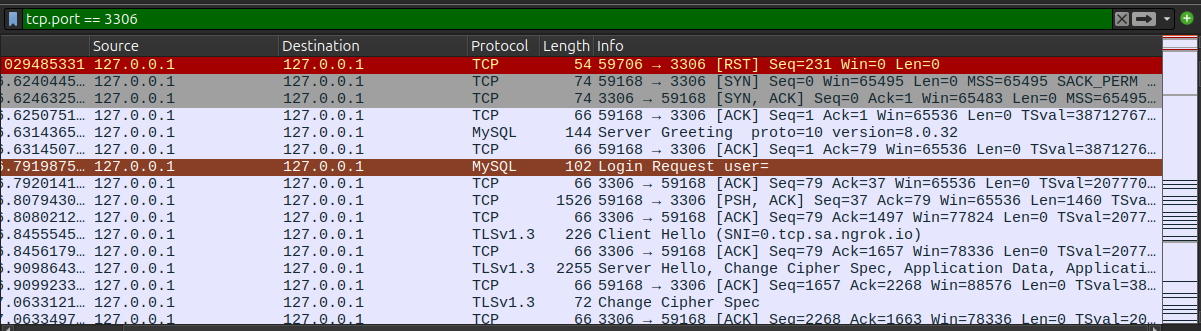
\includegraphics[width=\textwidth]{Captura de pantalla 2026-11-09 212930.png}
    \caption{Registro del logeo exitoso.}
    \label{fig:b1}
\end{figure}

\begin{figure}[hbt!]
    \centering
    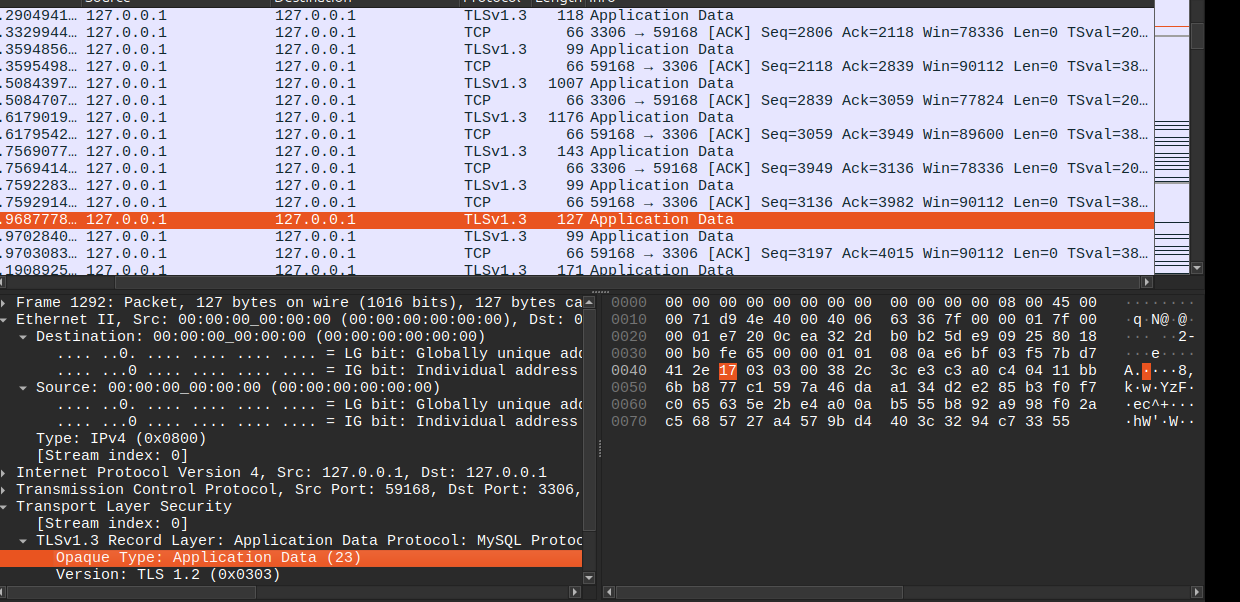
\includegraphics[width=\textwidth]{Captura de pantalla 2026-11-09 213210.png}
    \caption{Registro de la instrucción SQL filtrada.}
    \label{fig:b2}
\end{figure}

\subsection*{Anexo C. Consultas SQL empleadas}
En el cliente se documentaron las siguientes instrucciones como parte de la sesión de prueba:
\begin{lstlisting}
SHOW DATABASES;
SHOW TABLES FROM db_redes;
USE db_redes;
CREATE TABLE alumnos (
    id INT PRIMARY KEY,
    nombre VARCHAR(50),
    carrera VARCHAR(50)
);
\end{lstlisting}

\end{document}
